\documentclass[11pt, oneside]{article}   	% use "amsart" instead of "article" for AMSLaTeX format
\usepackage{geometry}                		% See geometry.pdf to learn the layout options. There are lots.
\geometry{letterpaper}                   		% ... or a4paper or a5paper or ... 

\usepackage{graphicx}				% Use pdf, png, jpg, or eps§ with pdflatex; use eps in DVI mode
								% TeX will automatically convert eps --> pdf in pdflatex		
\usepackage{amssymb}

%\usepackage{gb4e}
%\usepackage{enumitem}
%\usepackage{cancel}
\usepackage{amsmath}

\usepackage{mhchem}

\newcommand{\chemname}{Whitehorsehallium }

\title{Contrived Example Lab: Density of Liquid \chemname as a Function of Temperature}
\author{Mark Peever\\ \texttt{mpeever@gmail.com}}
\date{2025-09-09}							% Activate to display a given date or no date

\begin{document}
\maketitle

\section{Overview}
The purpose of this experiment is to determine the relationship between temperature and density of liquid \chemname at temperatures under $60^{\circ}C$. 
Density is found by measuring the volume of a given mass of \chemname at various temperatures.
The expectation is that the density of \chemname will decrease as temperature increases.

\section{Equipment List}
\begin{itemize}
\item handheld infrared thermometer
\item scale calibrated in grams
\item graduated cylinder
\item Erlenmeyer flask
\item bunsen burner
\end{itemize}

\section{Procedure}
A $50 mL$ sample of \chemname  was measured into a graduated and weighed to determine its mass.
The temperature of the sample was recorded, along with its volume and mass.

After measuring the sample's temperature, volume, and mass, the sample was poured into an Erlenmeyer flask and heated slowly over the bunsen burner.
The sample was stirred frequently by swishing the Erlenmeyer flask to ensure the temperature was even throughout, and temperature was monitored with the infrared thermometer.

At intervals of $10^{\circ}C$, the sample was poured into the graduated cylinder and weighed on the scale. The volume, mass, and temperature were recorded.

The sample was heated from $10^{\circ}C$ to $50^{\circ}C$.

\section{Observations and Data}
In the beginning, the sample appeared almost opaque. As the temperature increased, it became less opaque until it was almost clear at $34^{\circ}C$.
The sample's opacity did not visibly change above $34^{\circ}C$.

Measured temperature, volume, and mass of \chemname are given in Table \ref{table:sampleTable}.

\begin{table}[p]
\centering
\caption{Measured volumes of \chemname at various temperatures}
\begin{tabular}[b]{l | l| l}
\hline
Temperature & Volume & Mass \\
\hline
$10^{\circ} C$ & $50mL$   & $12 g$ \\
$20^{\circ} C$ & $60mL$   & $12 g$ \\
$30^{\circ} C$ & $70mL$   & $12 g$ \\
$40^{\circ} C$ & $78mL$   & $11.9 g$ \\
$50^{\circ} C$ & $88mL$   & $11.9 g$ \\
\end{tabular}
\label{table:sampleTable}
\end{table}

The density of the sample at each temperature is calculated as $\rho = \frac{mass}{Volume}$.
A graph of Volume vs. Temperature is given in Figure \ref{figure:sampleChart1}.
A graph of Density vs. Temperature is given in Figure \ref{figure:sampleChart2}.

\begin{figure}[p]
\centering
\caption{Volume vs. Temperature}
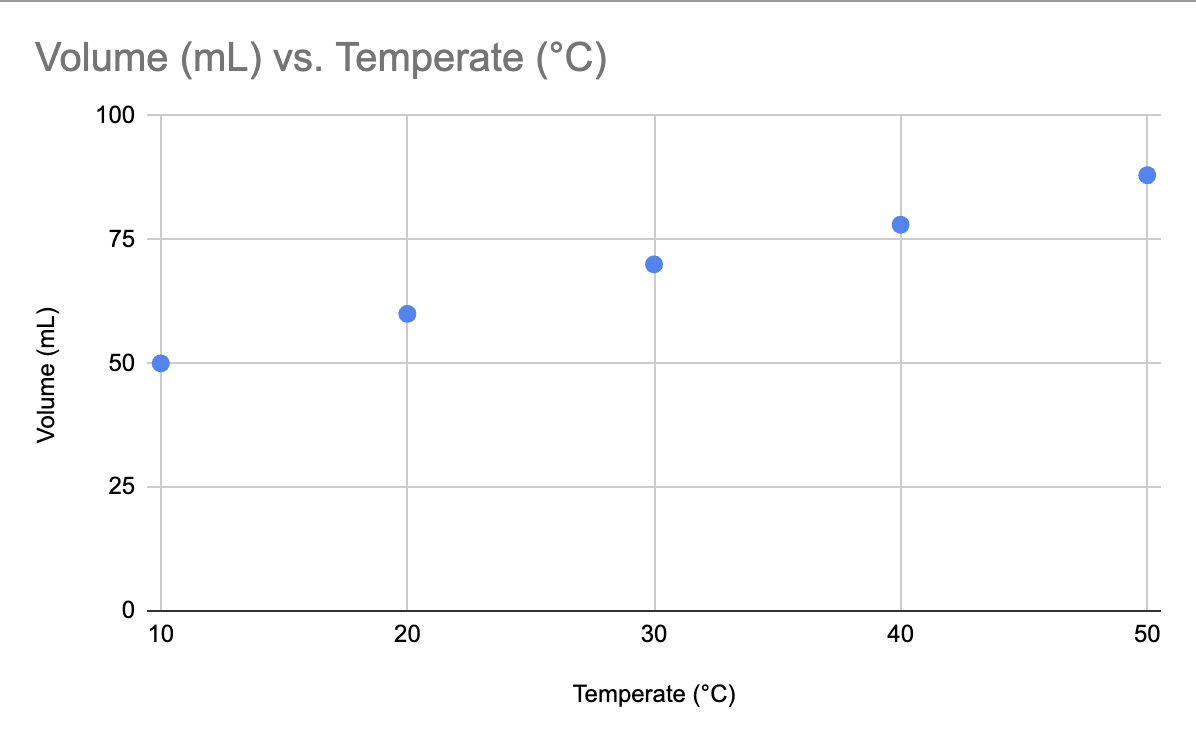
\includegraphics[scale=0.5]{Sample_Lab_Chart_1.png}
 \label{figure:sampleChart1}
 \end{figure}  

\begin{figure}[p]
\centering
 \caption{Density vs. Temperature}
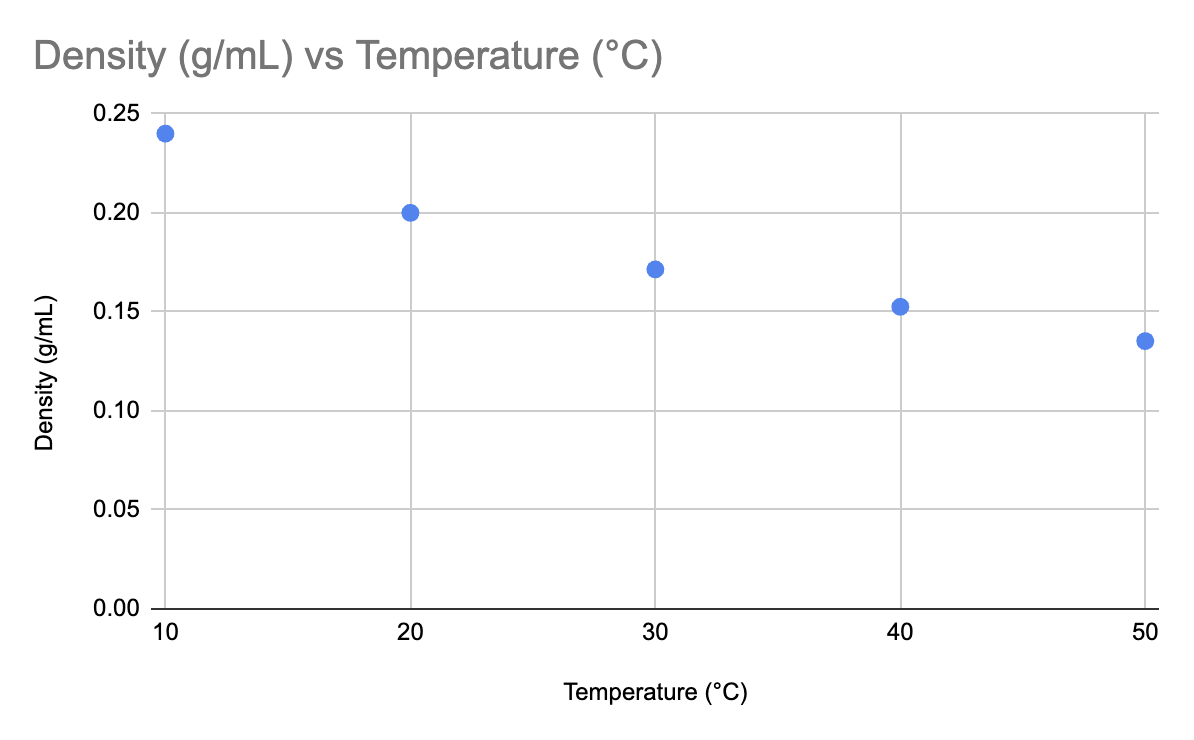
\includegraphics[scale=0.5]{Sample_Lab_Chart_2.png}
 \label{figure:sampleChart2}
 \end{figure}  

\section{Calculations}

\subsection{Sample Density Calculation}
 \begin{equation}
 \boxed{
\begin{split}
       T &= 10^{\circ}C & m &= 12 g & V &=  50mL \\
       \\
  	\rho &= \frac{m}{V} \\
	       &= \frac{12 g}{50 mL} \\
	       &= 0.24 \frac{g}{mL} \\
	       &= 0.2 \frac{g}{L} 
 \end{split}
 }
 \end{equation}
 
 \subsection{Density as a function of Temperature}
 \begin{itemize}
 \item slope of the line
 \begin{equation}
 \boxed{
\begin{split}
           m &= \frac{y_1 - y_0}{x_1 - x_0} \\
               &= (\frac{0.1352 \frac{g}{mL} - 0.24 \frac{g}{mL}}{50^{\circ}C - 10^{\circ}C}) \\
               &= -2.619 \times 10^{-3} \frac{g}{ml \cdot ^{\circ}C}
 \end{split}
 }
 \end{equation}
 
 \item $y$-intercept of the line
  \begin{equation}
 \boxed{
\begin{split}
             m &= \frac{y_1 - y_0}{x_1 - x_0} \\
             y &= mx + b \\
             b &= y_0 - m x_0 \\
                &= (0.24 \frac{g}{mL}) - (-2.619 \times 10^{-3} \frac{g}{ml \cdot ^{\circ}C})(10 ^{\circ}C) \\
                &= 0.2138 \frac{g}{mL}
 \end{split}
 }
 \end{equation}

\item equation of the line (density as a function of temperature)
  \begin{equation}
 \boxed{
\begin{split}
             y &= mx + b \\
             \rho &= (-2.619 \times 10^{-3} \frac{g}{ml \cdot ^{\circ}C}) T_C +  0.2138 \frac{g}{mL}\\
             \rho &= (-3 \times 10^{-3} \frac{g}{ml \cdot ^{\circ}C}) T_C +  0.2 \frac{g}{mL}\\
 \end{split}
 }
 \end{equation}
 \end{itemize}
 
 \section{Conclusion}
 The density of \chemname as a function of temperature was found to be given by the formula:
 $$ \rho &= (-3 \times 10^{-3} \frac{g}{ml \cdot ^{\circ}C}) T_C +  0.2 \frac{g}{mL} $$
 
 The final two samples were slightly smaller by mass than the first four. This might have affected the final outcome, making the final densities slightly smaller than expected.
 
 The temperature and volume measurements were only measured to one significant figure, which reduced the precision of this experiment.
 Another test with more precise measurements would find a more precise relationship.

\end{document}  